\section{Process Management and Deployment}\label{sec:pm}
In a production environment, many instances of a NodeJS server are run on
one machine; this way NodeJS applications can make use of multiple
processors. For this purpose, research into \emph{process managers} ---
applications used for running and managing production-level systems ---
was carried out.

\subsection{Process Manager Selection}\label{sec:pms}
A number of process managers were investigated with the hope of
incorporating them into the production
system~\cite{strongloop}\cite{pm2}\cite{forever}. The application pm2 was
chosen, primarily for its highly-configurable \emph{ecosystem}-config files,
and \emph{pmx}\footnote{https://github.com/keymetrics/pmx},
its profiling extension.

\subsection{pm2 and KeyMetrics}\label{sec:pm2}

\begin{figure}
	\centering
	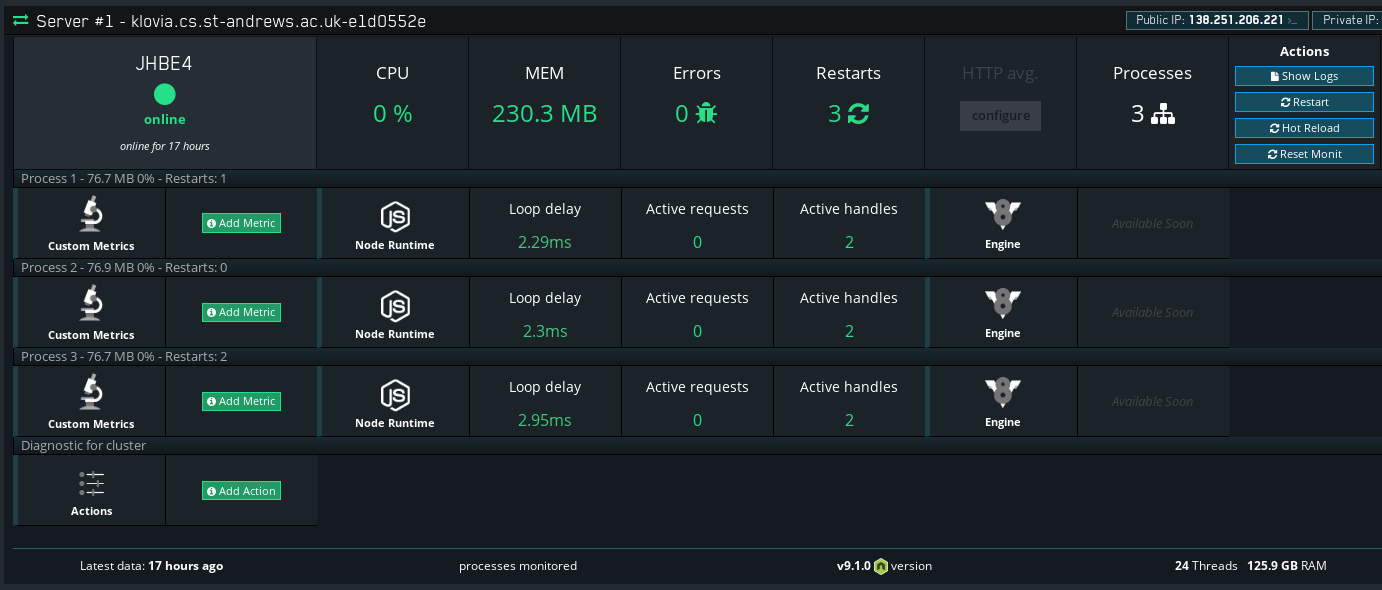
\includegraphics[width=0.95\linewidth]{km-dash}
	\caption{The KeyMetrics dashboard web client in use.}\label{fig:dash}
\end{figure}

A feature available in \emph{pm2} is the ability to transmit profiling
statistics to a web client, as a dashboard. The dashboard also allows the
user to remotely issue commands to the running instances. Further,
custom profiling information, and custom remote commands, can be created
through the introduction of simple logic into the codebase.

\subsection{Process Limitations}\label{sec:plim}
Running multiple NodeJS instances can quickly accumulate counts towards a
user process limit: each instance hosts several threads, and each connection
to the PostgreSQL database can pool several threads also, resulting in many
threads per instance. Compounded with the fact that pm2 itself also runs
as a NodeJS instance, this means that a user can reach their process limit
on the host labs very quickly. Using \texttt{nolimit} on process
instantiation is one solution, however this means having to run
\texttt{nolimit} when starting the databse, deamonising the process manager,
starting the server instances, and doing any miscellaneous tasks. This
limitation has stunted hindered attempts to connect to other teams'
products.

\subsection{Heroku Hosting}\label{sec:her}
In response to the issues addressed in \S\ref{sec:plim}, an attempt to host
an instance of the server on hosting service
\emph{Heroku}\footnote{https://heroku.com/} has been started. This would
alloow the team to interact with other teams, without using a member's
process limit and hindering their productivity. Additionally, it would show
the deployability of the system --- an important factor for a backend
server.

\subsection{External System Hosting}\label{sec:ext}
Another option is to host instances of the system on devices personally
owned by members of the team. This would give the team absolute control over
configuration of the sytem, and would have the potential to outperform an
instance running on a complementary Heroku service.
